\documentclass[11pt]{article}

%%%%%%%%%%%%%%Include Packages%%%%%%%%%%%%%%%%%%%%%%%%%%
\usepackage{xcolor}
\usepackage{mathtools}
\usepackage[a4paper, total={6in, 8in}, margin=1.25in]{geometry}
\usepackage{amsmath}
\usepackage{amssymb}
\usepackage{paralist}
\usepackage{rsfso}
\usepackage{amsthm}
\usepackage{wasysym}
\usepackage[inline]{enumitem}   
\usepackage{hyperref}
\usepackage{tocloft}
\usepackage{titlesec}
\usepackage{colortbl}
\usepackage{wrapfig}
\usepackage{pdfpages}
%%%%%%%%%%%%%%%%%%%%%%%%%%%%%%%%%%%%%%%%%%%%%%%%%%%%%%%%



\begin{document}
\Large \noindent \textbf{Physics 5A Final Review Session}\\
\normalsize
Department of Physics and Astronomy, UCLA\\
\noindent\rule{8cm}{0.4pt}\\

\noindent\textbf{Problem 1}: A solid sphere starts at rest from the top of a track, then rolls without slipping down the track. We are trying to stop the sphere at the bottom of the track using a huge spring. Neglect air friction in this problem. 
\begin{center}
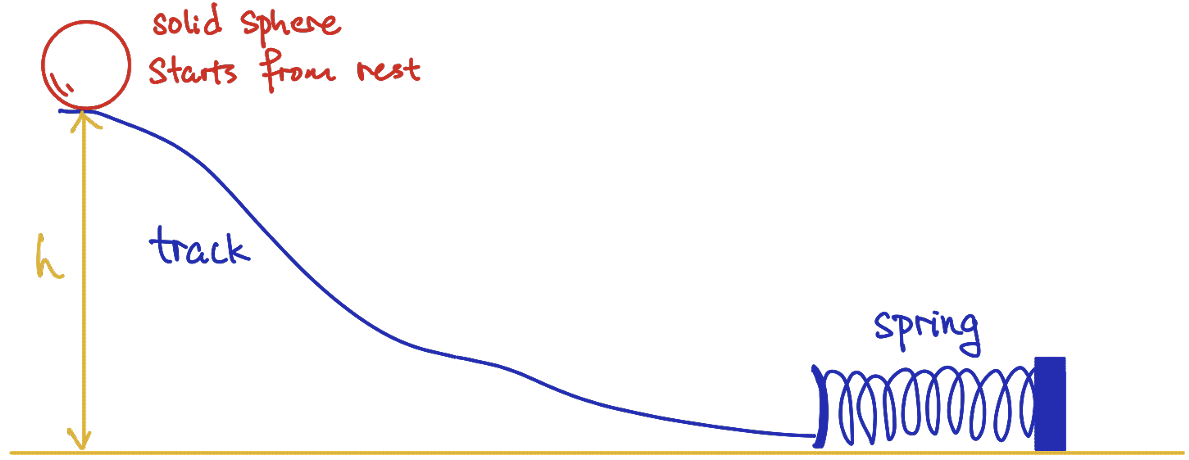
\includegraphics[scale=0.35]{sphere}
\end{center}

\noindent\textbf{Part (a)}: The sphere is rolling without slipping, what type of friction is involved?\\
\noindent\textbf{Part (b)}: What types of energy are involved in this process?\\

\noindent\textbf{Part (c)}: The sphere has mass $m$, the top of the track is at height $h$ above the ground. The spring has a spring constant $k$. The moment of inertia of a solid sphere is $I =(2/5) mr^2$ where $r$ is the radius of the sphere. Find symbolically the displacement from equilibrium of the spring that we need to stop the sphere at the bottom of the track, write it in terms of the variables given in the problem.\\

\noindent Now suppose a small loop is added to the track as shown. The top of the loop is at a height $d$ above the ground. 
\begin{center}
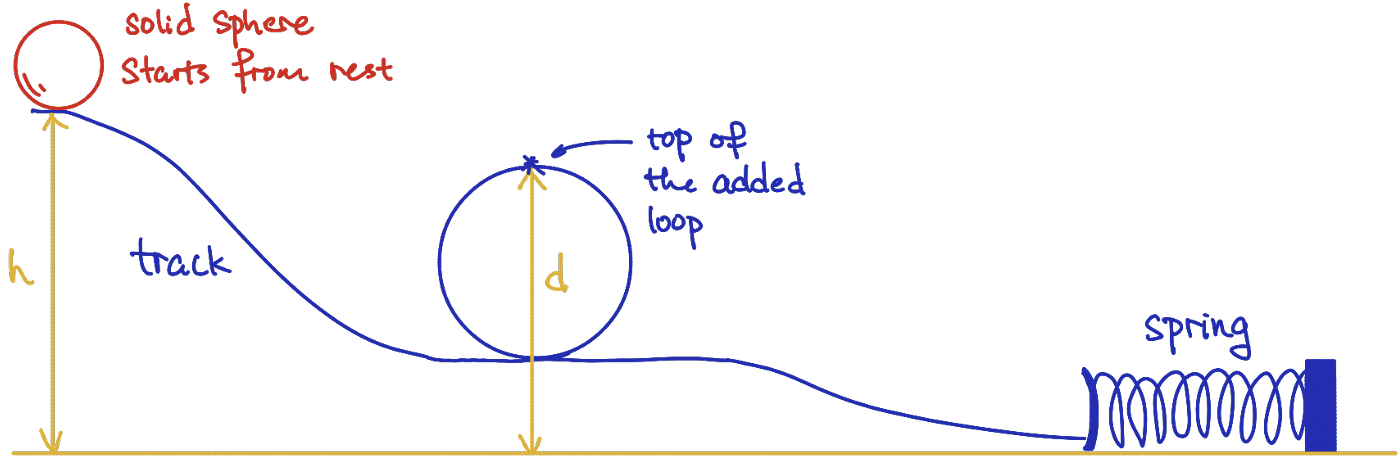
\includegraphics[scale=0.35]{loop.png}
\end{center}


\noindent\textbf{Part (d)}: Assuming that the sphere can go through the loop without falling off in the middle. (You should review the midterm 2 review session worksheet about the condition that the sphere being able to go through the loop without falling off. There is a minimum speed that the ball need to have when going through the loop.) Using conservation of energy, find symbolically the speed of the sphere when it gets to the top of the loop. \\

\noindent\textbf{Part (e)}: With the loop included in the track, find the displacement from equilibrium of the spring that we need to stop the sphere at the bottom of the track.\\

\noindent\textbf{Part (f)}: In this entire process, when does the system have the largest potential energy? When does the system have the largest kinetic energy?

\newpage
\noindent\textbf{Problem 2}: Jinyan is playing tennis. He hits the tennis ball with a racquet, giving the ball an initial velocity with magnitude $v_0$, in a direction $\theta=30^\circ$ above the ground. When the ball is hit, it is at $0.5$ meters above the ground. He wants the ball to be able to go over the $1$ meter tall tennis net that is $5$ meters away from where he hits the ball. What is the magnitude of the initial velocity $v_0$ that the ball should have in order to just barely go over the net (neglect the radius of the ball, treating it as a point-like particle)?

\begin{center}
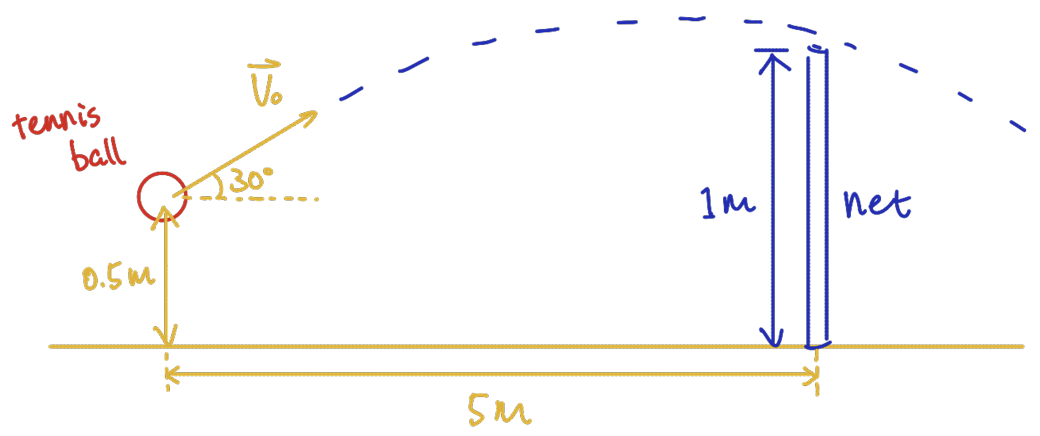
\includegraphics[scale=0.38]{tennis}
\end{center}


\newpage
\noindent\textbf{Solutions to problem 1}:\\
\noindent Part (a) - There are only two types of friction, kinetic friction and static friction. Kinetic friction applies when one surface is sliding over another one, such as a box sliding on the ground. Static friction applies when two surfaces are relatively stationary, such as a non-moving box on an incline. For rolling without slipping, the contact point of the sphere is instantaneously at rest relative to the surface of the track, the two surfaces are not sliding over each other, so static friction applies, kinetic friction does not apply.\\

\noindent Part (b) - The sphere itself is moving in space, including translational motion and rotational motion, so there are translational kinetic energy
\begin{align*}
T_t =\frac{1}{2} mv^2
\end{align*}
and rotational kinetic energy 
\begin{align*}
T_r = \frac{1}{2}I \omega^2\,.
\end{align*}
The sphere is going up and down in space, so we have to include gravitational potential energy 
\begin{align*}
U_g = mgh
\end{align*}
in our analysis. Finally, there is a spring at the end of the track, so we also need to consider spring potential energy
\begin{align*}
U_k = \frac{1}{2}k(\Delta x)^2\,.
\end{align*}

\noindent Part (c) - We start with the statement of conservation of energy,
\begin{align*}
(\text{initial energy})+ (\text{work done by external force}) = (\text{final energy})\,.
\end{align*} 
Only static friction is involved, but it does not do any work to the system in this case because the point of contact between the sphere and the surface has zero relative velocity. The gravitational force does do work to pull the sphere down, and the spring does do work to stop the sphere, but those effects have been included in $U_g$ and $U_k$, and they are not counted as "external" force in this problem. There is no other force presenting here, so work done by external force is zero. Breaking down the initial energy and final energy, we have
\begin{align*}
\frac{1}{2}mv_i^2 + \frac{1}{2}I\omega_i^2 + mgh_i =
\frac{1}{2}mv_f^2 + \frac{1}{2}I\omega_f^2 + mgh_f + \frac{1}{2}k(\Delta x)^2\,. 
\end{align*}
Now we know that the initial velocity is zero when the sphere is at the top of the track, so $v_i = 0$. The sphere rolls without slipping, so $\omega_i = v_i/r = 0$. At its final position, the sphere stops and so $v_f = 0$, rolling-without-slipping condition gives $\omega_f =v_f/r = 0$. Final height is $h_f = 0$ on the ground, and initial height is $h_i = h$. Thus we see
\begin{align*}
mgh = \frac{1}{2}k(\Delta x)^2\,,
\end{align*}
from which we find
\begin{align*}
\Delta x = \sqrt{2mgh/k}\,.
\end{align*}


\noindent Part (d) - Again we start with conservation of energy, but the spring energy is not relevant for this part because the sphere haven't got to the spring yet. 
\begin{align*}
\frac{1}{2}mv_i^2 + \frac{1}{2}I\omega_i^2 + mgh_i =
\frac{1}{2}mv_f^2 + \frac{1}{2}I\omega_f^2 + mgh_f\,.
\end{align*}
This time, we pick the initial point to be at the top of the track (where the sphere starts its motion) and the final point to the bat the top of the loop. Again, we know that $v_i = 0$ and $\omega_i = 0$ at the moment the sphere starts rolling. The initial height is $h_i = h$ and the final height is $h_f = d$, so we have
\begin{align*}
mgh = \frac{1}{2}mv_f^2 + \frac{1}{2}I\omega_f^2 + mgd\,.
\end{align*}
As given in the problem, we have $I = (2/5) mr^2$, and the rolling-without-slipping condition gives $\omega_f = v_f/r$, so we can use them to get
\begin{align*}
mgh =
\frac{1}{2}mv_f^2 + \frac{1}{2}\left(\frac{2}{5}mr^2 \right)\left(\frac{v_f}{r}\right)^2 + mgd
\end{align*}
and we can simplify the right-hand side of the equation to get
\begin{align*}
mgh = \frac{1}{2}mv_f^2 + \frac{1}{5}m v_f^2 + mgd = \frac{7}{10}mv_f^2 + mgd\,.
\end{align*}
The speed of the sphere when it gets to the top of the loop is 
\begin{align*}
v_f =\sqrt{\frac{10}{7m} ( mgh-mgd)} = \sqrt{\frac{10 g (h-d)}{7}}\,.
\end{align*}
Let us also review the condition that the sphere can stay on the track without falling off when going through the loop. We expect to see the sphere to be moving the slowest when it gets to the top of the loop. If it goes too slow at the top, it will just fall down and being unable to maintain the circular motion. We only have downward normal force and downward gravitational force acting on the sphere, and the sum of the two is the downward centripetal force that we want when the sphere is at the top of the loop. The "threshold" happens when the downward normal force disappear, so 
\begin{align*}
-mg = -\frac{mv_{\min}^2}{R}\,,
\end{align*}
and this is 
\begin{align*}
v_{\min} = \sqrt{gR}\,.
\end{align*}
If the sphere goes slower than this at the top of the loop, it will lose contact with the track and fall down. In this analysis, I have assumed that $R$ is much larger than the radius of the sphere and thus I have neglected the effect of $r$ in my calculation.\\


\noindent Part (e) - Even with the loop included in the track, the displacement of the spring is still the one we found in part (c), 
\begin{align*}
\Delta x = \sqrt{2mgh/k}\,.
\end{align*}
This is because the way we setup conservation of energy will be the same as in part (c), we do not care about any intermediate process that the sphere will go through when setting up the conservation of energy. We only need to pick the initial point (at the top of the track) and the final point (at the bottom of the track) when solving this problem. You might argue that, the sphere has traveled a little longer in this part when going through the loop, maybe that will slow down the sphere a little bit? And maybe that will result in a smaller displacement of the spring to stop the sphere? This is not correct because we have neglected the air friction and other frictions that will slow down the sphere when it is traveling. If we have included those in our analysis, those frictions contribute external work and will slow down the sphere if the sphere has traveled a longer distance. However, in our analysis, the static friction that maintain the rotational motion of the sphere never slows down the sphere. \\

Part (f) - In this process, the sphere is the one that has kinetic energy, and kinetic energy is the largest when the sphere is moving the fastest, because
\begin{align*}
T = \frac{1}{2}mv^2 + \frac{1}{2}I\omega^2\,,
\end{align*}
the larger the $v$ and $\omega$, the larger the $T$. The sphere is moving the fastest right before it hits the spring (which will slow it down), so right before the sphere hits the spring, the system has the largest kinetic energy. The kinetic energy and potential energy of the system sum up to the total energy, which is conserved in the process because there is no external work done. Therefore, if kinetic energy is low, potential energy must be high. The potential energy is thus the highest when the sphere is not moving, this corresponds to the starting point when the sphere is at the top of the track, and the ending point when the sphere is stopped by the spring. The former one corresponds to all energy being stored in gravitational potential energy of the sphere, and the later one corresponds to all energy being stored in the potential energy of the spring.\\

 

\textbf{Problem 2}: Problem 2 should be easier here. You should review midterm 1 review session worksheet if you want to see more details. At any time $t$, we can find the location of the tennis ball using
\begin{align*}
y = \frac{1}{2}a_y t^2 + v_{0,y}t  + y_0\,,\\
x = \frac{1}{2}a_x t^2 + v_{0,x}t  + x_0\,.
\end{align*}
Then we plug in the numbers. Here $a_y = -9.8$, $v_{0,y} = v_0 \sin(30^\circ)$, $y_0 = 0.5$, $a_x = 0$, $v_{0,x} = v_0 \cos(30^\circ)$, and $x_0 = 0$. In particular, we want to first compute the time that the ball can get to the net. The net is $5$ meters away from where the ball is hit, so we set $x = 5$, and use the second equation 
\begin{align*}
5 = v_0 \cos(30^\circ) t
\end{align*}
to get the time
\begin{align*}
t = \frac{5}{v_0 \cos(30^\circ)}\,.
\end{align*}
This is the time it takes from the ball to travel from where it gets hit to somewhere above or below the net. Now we want the ball to be able to barely go over the net, which is $1$ meter tall, so we set $y = 1$ meter at time $t = 5/(v_0 \cos(30^\circ))$. That is, 
\begin{align*}
1 = \frac{1}{2}(-9.8) \left( \frac{5}{v_0 \cos(30^\circ)}\right)^2 + \left(v_0 \sin(30^\circ) \right)\left(\frac{5}{v_0 \cos(30^\circ)}\right) + 0.5\,.
\end{align*} 
This allows us to find $v_0$, you should get
\begin{align*}
v_ 0 =8.27\,\text{m/s}\,.
\end{align*}

\end{document}


